
\chapter{Approach to Molecular Solvents\label{chpt:iem-mdft}}

We now consider the case of a non-spherical molecular solvent, like
water. The solvent molecules now carry a molecular structure that
is described by a collection of distributed atomic interaction sites
(LJ and Coulombic). The two theories mentioned in the previous section
are formulated in the molecular picture in which each solvent molecule
is considered as a rigid body and characterized by its position, $\mathbf{r}$
(e. g. the position of center of mass), and its orientation, $\mathbf{\Omega}$,
defined by the three Euler angles $\mathbf{\Omega}\equiv(\Theta,\Phi,\Psi)$.
In \acs{MDFT}, the solvent is characterized by an inhomogeneous position
and orientation density $\rho(\mathbf{r},\mathbf{\Omega})$. In \acs{IET},
an angular dependent form of the pair distribution function $g(\mathbf{X}_{1},\mathbf{X}_{2})$
($X\equiv(\mathbf{r},\mathbf{\Omega})$) is proposed, and the molecular
\acs{OZ} equation is expanded on rotational invariants. Another way
to extend the IET is the RISM \citep{hirata_molecular_2004} which
will not be discussed in this thesis.

\section{Molecular density functional theory}

Here we can just extend some equations written in the last section
to the case of an angular-dependent external potential and density.
In \acf{MDFT}, the grand potential density functional corresponding
to an inhomogeneous fluid density $\rho(\mathbf{r},\mathbf{\Omega})$
is given by (changing notations not to confuse the traditional notation
of the grand potential with that of the orientations):
\begin{equation}
\Theta[\rho(\mathbf{r},\mathbf{\Omega})]=\Theta[\rho_{0}]+\mathcal{F}[\rho(\mathbf{r},\mathbf{\Omega})]
\end{equation}
where $\Theta[\rho_{0}]$ is the correspondent reference bulk fluid
grand potential and $\rho$ is the fluid density function depending
now on 5 or 6 variables, 3 coordinates of the positions, and 2 or
3 for the angular part depending on whether the molecule is linear or not.
The homogeneous density is equal to $n_{0}/4\pi$for a linear solvent, and
$n_{0}/8\pi^{2}$ for the general case.

According to the variation principle described above, the equilibrium
density can be found by minimizing the free energy functional $\mathcal{F}[\rho]$
regarding to $\rho(\mathbf{r},\mathbf{\Omega})$:
\begin{equation}
\left.\frac{\delta\mathcal{F}[\rho]}{\delta\rho(\mathbf{r},\mathbf{\Omega})}\right|_{\rho=\rho_{0}}=0
\end{equation}

This functional is defined as a sum of functional contributions:
\begin{equation}
\mathcal{F}[\rho]=\mathcal{F}_{\mathrm{id}}[\rho]+\mathcal{F}_{\mathrm{ext}}[\rho]+\mathcal{F}_{\mathrm{exc}}[\rho]\label{eq:fff}
\end{equation}


\subsection{The ideal term}

The ideal term $\mathcal{F}_{\mathrm{id}}[\rho]$ is deduced from
the particle interaction-free condition: 
\begin{equation}
\mathcal{F}_{\mathrm{id}}[\rho]=\beta^{-1}\int\mathrm{d}\mathbf{r}\mathrm{d\Omega}\left[\mathbf{\mathbf{\ln\left(\frac{\rho(\mathbf{r},\mathbf{\mathbf{\mathbf{\mathbf{\Omega}}}})}{\rho_{0}}\right)}}-\rho(\mathbf{r},\mathbf{\mathbf{\mathbf{\Omega}}})+\rho_{0}\right]
\end{equation}
where $\rho_{0}$ is the reference bulk density of pure solvents. The
differentiation of $\mathcal{F}_{\mathrm{id}}[\rho]$ will be used
for the minimization, discussed later, which has form
\begin{equation}
\frac{\delta\mathcal{F}_{\mathrm{id}}[\rho]}{\delta\rho(\mathbf{r},\mathbf{\Omega})}=\beta^{-1}\ln\left(\dfrac{\rho(\mathbf{r},\mathbf{\Omega})}{\rho_{0}}\right)
\end{equation}


\subsection{The external term}

The solute, like the solvent, is described in microscopic detail by
a molecular non-polarizable force field involving atomic Lennard-Jones
and partial charge parameters, creating at each point in space an
external potential ($V_{\mathrm{ext}}(\mathbf{r},\mathbf{\mathbf{\mathbf{\mathbf{\Omega}}}})$),
containing two components:
\begin{equation}
V_{\mathrm{ext}}(\mathbf{r},\mathbf{\Omega})=V_{\mathrm{LJ}}(\mathbf{r})+V_{\mathrm{coul}}(\mathbf{r},\mathbf{\Omega})
\end{equation}

The external potential term calculates the contribution of $V_{\mathrm{ext}}$:
\begin{equation}
\mathcal{F}_{\mathrm{ext}}[\rho]=\int\mathrm{d}\mathbf{r}\mathrm{d}\mathbf{\mathbf{\Omega}}V_{\mathrm{ext}}(\mathbf{r},\mathbf{\mathbf{\mathbf{\mathbf{\Omega}}}})\rho(\mathbf{r},\mathbf{\mathbf{\mathbf{\mathbf{\Omega}}}})
\end{equation}

The Lennard-Jones potential is given by
\begin{equation}
V_{\mathrm{LJ}}(\mathbf{r})=\sum_{u}\sum_{v}4\epsilon_{uv}\left[\left(\dfrac{\sigma_{uv}}{r_{uv}}\right)^{12}-\left(\dfrac{\sigma_{uv}}{r_{uv}}\right)^{6}\right]\label{eq:LJ}
\end{equation}

where $u$ stands for solute, $v$ stands for solvent, $\epsilon_{uv}=\sqrt{\epsilon_{u}\epsilon_{v}}$
and $\sigma_{uv}=\left(\sigma_{u}+\sigma_{v}\right)$ are the geometric
and arithmetic average Lennard-Jones parameters between solute and
solvent, according to the Lorentz-Berthelot mixing rules. $r_{ij}$
is the norm of relative site-site vector
\begin{equation}
\mathbf{r}_{uv}=\mathbf{r}+\mathbf{R}(\mathbf{\Omega})\mathbf{s}_{v}-\mathbf{r}_{u}\label{eq:ruv}
\end{equation}
where $\mathbf{r}_{u}$ and $\mathbf{s}_{j}$ are the coordinates
of solute/solvent molecules in the molecular frame, and $\mathbf{R}(\mathbf{\Omega})$
is the rotation matrix of the Euler angles $\mathbf{\Omega}$.

In cases where the solvent site wears only one LJ centre, eq. (\ref{eq:ruv})
reduces to

\begin{equation}
\mathbf{r}_{uv}=\mathbf{r}-\mathbf{r}_{u}
\end{equation}
which is actually what we use in the code as the solvent is SPC/E
water.

The Coulomb interaction is calculated by \textcolor{red}{solving the
Poisson equation \citep{Marchi_2001}.} The charge density of the
solute is projected onto a space grid,
\begin{equation}
\rho_{q}(\mathbf{r})=\sum_{u}q_{ijk}
\end{equation}
where $q_{ijk}$ is the charge on the space grid distributed by its
nearby point charge as shown in figure \ref{fig:Charge-density-projected}
(a).

\begin{figure}[h]
\begin{centering}
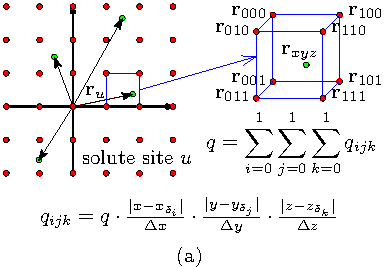
\includegraphics{_figure/charge_int}
\par\end{centering}
\caption{Charge density projected onto grids\label{fig:Charge-density-projected}.
(a) Solute. (b) Solvent.}
\end{figure}

\begin{equation}
V_{\mathrm{coul}}(\mathbf{r},\mathbf{\Omega})=\sum_{v}q_{v}V_{q}(\mathbf{r}_{u})
\end{equation}
where $V_{q}(\mathbf{r})$ is the electrostatic potential created
by the charge distribution $\rho_{q}(\mathbf{r})$. It can be computed
using a periodic Poisson Solver. The Poisson equation reads

\begin{equation}
\nabla^{2}V_{q}(\mathbf{r})=-\frac{\rho_{q}(\mathbf{r})}{\varepsilon_{0}}
\end{equation}

or in Fourier space
\begin{equation}
\hat{V}_{q}(\mathbf{k})=\frac{\hat{\rho}_{q}(\mathbf{k})}{\varepsilon_{0}k^{2}}
\end{equation}
where $\hat{V}_{q}(\mathbf{k})$, $\hat{\rho}_{q}(\mathbf{k})$ are
the Fourier transform of $V_{q}(\mathbf{r})$, $\rho_{q}(\mathbf{r})$
respectively. $\rho_{q}(\mathbf{r})$ is transformed forward, $\hat{V}_{q}(\mathbf{k})$
is computed and transformed backward. $V_{q}(\mathbf{r}_{u})$ is
then obtained by interpolation. 

\subsection{The excess term}

The two terms $\mathcal{F}_{\mathrm{id}}[\rho]$ and $\mathcal{F}_{\mathrm{ext}}[\rho]$
are physically exact, while the excess term $\mathcal{F}_{\mathrm{exc}}[\rho]$
depends on the exact correlation function, which is a priori unknown.
As in the previous section, we invoke here the \acs{HRF} approximation
which amounts to a second-order Taylor expansion around the homogeneous
fluid at density $\rho_{0}$:
\begin{equation}
\mathcal{F}_{\mathrm{exc}}[\rho]=\frac{k_{B}T}{2}\int\mathrm{d}\mathbf{r_{1}}\mathrm{d}\mathbf{\mathbf{\Omega}}\gamma(\mathbf{r}_{1},\mathbf{\mathbf{\mathbf{\mathbf{\Omega}}}})\rho(\mathbf{r_{1}},\mathbf{\mathbf{\mathbf{\mathbf{\Omega}}}})\label{eq:fexc}
\end{equation}
where $\gamma$ is the normalized gradient of the excess functional:
\begin{equation}
\gamma(\mathbf{r_{1}},\mathbf{\Omega_{1}})=\frac{\delta\beta F_{\mathrm{exc}}}{\delta\rho}=-\int\mathrm{d}\mathbf{r_{2}}\mathrm{d}\mathbf{\Omega_{2}}\Delta\rho(\mathbf{r}_{2},\mathbf{\Omega}_{2})c(\mathbf{r}_{12},\mathbf{\Omega}_{1},\mathbf{\Omega}_{2})\label{eq:gamma}
\end{equation}

To evaluate the gradient $\gamma$ for each $\mathbf{(r},\mathbf{\Omega})$,
$N\equiv N_{\mathbf{r}}N_{\mathbf{\Omega}}$ function evaluations
(\acs{FE}) are required. The total number of \acs{FE} is thus $N^{2}=O(N^{2})$,
which, with typically $N_{\mathbf{r}}=64^{3}$ and $N_{\mathbf{\Omega}}=50\sim100$,
is far too costly for current computing technology. For this reason,
Fourier transform is used to treat the spatial convolution in eq.
(\ref{eq:gamma}).

A convolution
\begin{equation}
h(x_{1})\equiv f(x_{2})\otimes g(x_{2})\equiv\int_{a}^{b}f(x_{2})g(x_{1}-x_{2})dx_{2}\label{eq:convolution-1}
\end{equation}
has the property that
\begin{equation}
\mathfrak{F}[h(x_{1})]=\mathfrak{F}[f(x_{2})]\mathfrak{F}[g(x_{2})]\label{eq:convolution-2}
\end{equation}
$\mathfrak{F}$ being the Fourier transform operation. As $\mathbf{r_{12}}=\mathbf{r_{1}}-\mathbf{r_{2}}$,
eq. (\ref{eq:gamma}) is a 3D convolution, which leads to
\begin{equation}
\hat{\gamma}(\mathbf{k},\mathbf{\Omega_{1}})=-\beta^{-1}\int\mathrm{d}\mathbf{\Omega}_{2}\Delta\hat{\rho}(\mathbf{k},\mathbf{\Omega}_{2})\hat{c}(\mathbf{k},\mathbf{\Omega}_{1},\mathbf{\Omega}_{2})\label{eq:gamma-k}
\end{equation}

Thus the integral $\int\mathrm{d}\mathbf{r_{2}}$ in eq. (\ref{eq:gamma})
is transformed into a simple product in eq. (\ref{eq:gamma-k}). To
get $\hat{\gamma}(\mathbf{k},\mathbf{\Omega_{1}})$ with given $\Delta\hat{\rho}(\mathbf{k},\mathbf{\Omega_{2}})$,
only $N_{\mathbf{r}}N_{\mathbf{\Omega}}^{2}$\acs{FE} are needed.
To this computational cost should be added the transform from $\Delta\rho(\mathbf{r},\mathbf{\Omega})$
to $\Delta\hat{\rho}(\mathbf{k},\mathbf{\Omega})$ and the backward
transform from $\hat{\gamma}(\mathbf{k},\mathbf{\Omega})$ to $\gamma(\mathbf{r},\mathbf{\Omega})$
which are both of order $N_{\mathbf{\Omega}}\cdot O(N_{\mathbf{r}}\log_{2}N_{\mathbf{r}})$
due to the properties of Fast Fourier Transforms (\acs{FFT}). The
total number of \acs{FE} is thus reduced from quadratic complexity
$O(N_{\mathbf{r}}^{2}N_{\mathbf{\Omega}}^{2})$ to $N_{\mathbf{r}}N_{\mathbf{\Omega}}^{2}+2N_{\mathbf{\Omega}}\cdot O(N_{\mathbf{r}}\log_{2}N_{\mathbf{r}})=O(N_{\mathbf{r}}\log_{2}N_{\mathbf{r}}N_{\mathbf{\Omega}}^{2})$.
As the total number of spatial grid $N_{\mathbf{r}}$ is of magnitude
$10^{5}\sim10^{6}$, this procedure, which is mathematically equivalent
to the direct evaluation (\ref{eq:gamma}), offers a great advantage
in terms of computational efficiency (figure \ref{fig:order-of-growth}
in section \ref{chpt:introduction}).

Once $\gamma(\mathbf{r},\mathbf{\Omega})$ is obtained by inverse
Fourier transform of $\gamma(\mathbf{r},\mathbf{\Omega})$, the excess
functional can be calculated as eq. (\ref{eq:fexc}).

The input $\hat{c}(\mathbf{k},\mathbf{\Omega}_{1},\mathbf{\Omega}_{2})$
is an angular-dependent \acs{DCF} of the homogeneous solvent which
depends on the relative position of two molecules $r_{12}$ and their
orientations (two in the initial code \citep{Zhao_2011}, and three
developed in this thesis). This quantity is provided with high
precision and in different representations by Luc Belloni, using a
mixture of Monte-Carlo simulations and inversion of the angular-dependent
\acs{MOZ} equation within a rotational invariant expansion \citep{puibasset_bridge_2012}.
A detailed comparison of some \acs{DCF}s is in appendix \textcolor{red}{{[}ref{]}}.

\section{Angular dependent integral equation theory}

To extend the \acs{IET} formalism to molecular cases, Blum \citep{Blum_I,Blum_II}
proposed an angular-dependent form of the pair distribution function,
which is then used in the \acs{IET} formalism. Fries \& Patey \citep{Fries_Patey_1985}
proposed the numerical solution of the full \acs{HNC} theory using
angle-dependent pair potentials. The description below is based on
these articles.

The angular-dependent \acs{PDF} is defined as 
\begin{equation}
g(\mathbf{X}_{1},\mathbf{X}_{2})\equiv g(\mathbf{r}_{1},\mathbf{r}_{2},\mathbf{\Omega}_{1},\mathbf{\Omega}_{2})
\end{equation}
which possesses the translational invariance if the fluid is homogeneous:
\begin{equation}
g(\mathbf{X}_{1},\mathbf{X}_{2})=g(\mathbf{r}_{12},\mathbf{\Omega}_{1},\mathbf{\Omega}_{2})
\end{equation}
and the rotational invariance \textcolor{red}{(attention indices)}:
\begin{equation}
g(\mathbf{X}_{1},\mathbf{X}_{2})=\sum_{m,n,l=0}^{\infty}\sum_{\left|\mu,\mu'\right|\leq m,\left|\nu,\nu'\right|\leq m,\left|\lambda\right|\leq l}g_{\mu,\mu'\nu\nu'\lambda}^{mnl}(\left\Vert \mathbf{r}_{12}\right\Vert )R_{\mu\mu'}^{m}(\mathbf{\Omega}_{1})R_{\nu\nu'}^{m}(\mathbf{\Omega}_{2})R_{\lambda0}^{l}(\hat{\mathbf{r}}_{12})
\end{equation}

The suggestion of Wigner gives a set of rotation invariant:
\begin{equation}
\Phi_{\mu'\nu'}^{mnl}(\hat{\mathbf{r}}_{12},\mathbf{\Omega}_{1},\mathbf{\Omega}_{2})=f^{mnl}\sum_{\mu\nu\lambda}\left(\begin{array}{ccc}
m & n & l\\
\mu & \nu & \lambda
\end{array}\right)R_{\mu\mu'}^{m}(\mathbf{\Omega}_{1})R_{\nu\nu'}^{m}(\mathbf{\Omega}_{2})R_{\lambda0}^{l}(\hat{\mathbf{r}}_{12})
\end{equation}
such that
\begin{equation}
g(\mathbf{X}_{1},\mathbf{X}_{2})=\sum_{mnl}\sum_{\mu'\nu'}g_{\mu'\nu'}^{mnl}(\left\Vert \mathbf{r}_{12}\right\Vert )\Phi_{\mu'\nu'}^{mnl}(\hat{\mathbf{r}}_{12},\mathbf{\Omega}_{1},\mathbf{\Omega}_{2})
\end{equation}
and
\begin{equation}
g_{\mu'\nu'}^{mnl}=\sum_{\mu\nu\lambda}\left(\begin{array}{ccc}
m & n & l\\
\mu & \nu & \lambda
\end{array}\right)g_{\mu,\mu'\nu\nu'\lambda}^{mnl}
\end{equation}

The molecular Ornstein-Zernike \acs{MOZ} equation is defined as
\begin{equation}
h(\mathbf{X}_{1},\mathbf{X}_{2})-c(\mathbf{X}_{1},\mathbf{X}_{2})=\frac{\rho}{8\pi^{2}}\int\mathrm{d}\mathbf{X}_{3}h(\mathbf{X}_{1},\mathbf{X}_{3})c(\mathbf{X}_{3},\mathbf{X}_{2})
\end{equation}
which can be both expanded as
\begin{equation}
h(\mathbf{X}_{1},\mathbf{X}_{2})=\sum_{mnl}\sum_{\mu'\nu'}h_{\mu'\nu'}^{mnl}(\left\Vert \mathbf{r}_{12}\right\Vert )\Phi_{\mu'\nu'}^{mnl}(\hat{\mathbf{r}}_{12},\mathbf{\Omega}_{1},\mathbf{\Omega}_{2})
\end{equation}
\begin{equation}
c(\mathbf{X}_{1},\mathbf{X}_{2})=\sum_{mnl}\sum_{\mu'\nu'}c_{\mu'\nu'}^{mnl}(\left\Vert \mathbf{r}_{12}\right\Vert )\Phi_{\mu'\nu'}^{mnl}(\hat{\mathbf{r}}_{12},\mathbf{\Omega}_{1},\mathbf{\Omega}_{2})
\end{equation}
\begin{equation}
\eta(\mathbf{X}_{1},\mathbf{X}_{2})=h(\mathbf{X}_{1},\mathbf{X}_{2})-c(\mathbf{X}_{1},\mathbf{X}_{2})=\sum_{mnl}\sum_{\mu'\nu'}\eta_{\mu'\nu'}^{mnl}(\left\Vert \mathbf{r}_{12}\right\Vert )\Phi_{\mu'\nu'}^{mnl}(\hat{\mathbf{r}}_{12},\mathbf{\Omega}_{1},\mathbf{\Omega}_{2})
\end{equation}
As an analog to the \acs{FFT} the fast Hankel transform can deal
these rotational invariant projections into $k$-space, such that
\begin{equation}
\hat{c}_{\mu\nu}^{mnl}(k)=4\pi i^{l}\int\mathrm{d}r\,r^{2}j_{l}(kr)c_{\mu\nu}^{mnl}(r)
\end{equation}
\begin{equation}
\hat{\eta}_{\mu\nu}^{mnl}(k)=4\pi i^{l}\int\mathrm{d}r\,r^{2}j_{l}(kr)\eta_{\mu\nu}^{mnl}(r)
\end{equation}
where $j_{l}(kr)$ are the spherical Bessel functions.

The $\chi$-transform defined by Blum gives
\begin{equation}
\hat{c'}_{\mu\nu,\chi}^{mn}(k)=\sum_{l=\left|m-n\right|}^{m+n}\left(\begin{array}{ccc}
m & n & l\\
\chi & -\chi & 0
\end{array}\right)\hat{c}_{\mu\nu}^{mnl}(k)
\end{equation}
\begin{equation}
\hat{\eta'}_{\mu\nu,\chi}^{mn}(k)=\sum_{l=\left|m-n\right|}^{m+n}\left(\begin{array}{ccc}
m & n & l\\
\chi & -\chi & 0
\end{array}\right)\hat{\eta}_{\mu\nu}^{mnl}(k)
\end{equation}
If $\Phi_{\mu'\nu'}^{mnl}(\hat{\mathbf{r}}_{12},\mathbf{\Omega}_{1},\mathbf{\Omega}_{2})$
is defined with the factor $f^{mnl}=\left[(2m+1)(2n+1)\right]^{1/2},$
the \acs{MOZ} equation can be reduced by Blum's reduction such that
\begin{equation}
\hat{\eta'}_{\mu\nu,\chi}^{mn}(k)=\rho\sum_{n_{1}}\sum_{\nu_{1}=-n_{1}}^{n_{1}}(-)^{\chi+\nu_{1}}\left[\hat{\eta'}_{\mu\nu_{1},\chi}^{mn_{1}}(k)+\hat{c'}_{\mu\nu_{1},\chi}^{mn_{1}}(k)\right]\hat{c'}_{\underline{\nu_{1}}\nu,\chi}^{n_{1}n}(k)
\end{equation}
which reduces the calculation of $(\mathbf{X}_{1},\mathbf{X}_{3})$
for $(\mathbf{X}_{3},\mathbf{X}_{2})$ to a sum of $n_{1}$, $\nu_{1}$.

\textcolor{red}{(The part of HNC has non need in this thesis.)}
